\chapter{Architecture}
\label{cha:architecture}

In this chapter the architecture of the system will be exposed. The whole can be seen as a web service that exposes some REST API, and internally deals with social network interaction and data analysis. Firstly, a logical explaination of the process will be given, secondly the API will be officialy exposed, and finally a complete view on the architecture will be provided.

\section{Solution design}
\label{sec:design}
This section describes the specifications of the functionalities of the system. Each functionality is a logical group of actions whose purpose is to carry out a section of the job required to go from row data - a user identifier - to a piece of information - the answer to the question "Has this person lived a life event?". The steps are the following, as shown in figure~\ref{fig:nutshell}:
\begin{enumerate}
\item Collect activities from social networks.
\item Extract semantic entities from social network contents.
\item classify each content.
\item Decide whether the user has lived the life event relying on his/her contents.
\end{enumerate}
In the following subsections the logic of the proposed methodology will be illustrated, providing also a likely signature of each part. To do that, the concept of \textit{post} is now formalized in an object call \texttt{Post}: it includes all the useful data for this purpose, such as date of creation, number of likes and shares, sentiment score, entity and topic sets and the probability to be about a life event. At the beginning of the analysis many of this attributes will be empty, and each logical step will add a piece of information.\\

\begin{center}
\label{tab:post}
\begin{tabular}{lll}
\hline
Post & & \\
\hline
\textbf{Date} & created & \%The creation date of the post \\
\textbf{Integer} & likes & \%Number of likes received \\
\textbf{Integer} & shares & \%Number of shares \\
\textbf{Float} & sentiment & \%Sentiment score \\
\textbf{Set} & entities & \%Set of strings representing the entities found in post text or images \\
\textbf{Set} & topics & \%Set of strings representing the topics found in post text or images \\
\textbf{Float} & probability & \%Probability of the post to be about a life event \\
\hline
\end{tabular}
\end{center}


\begin{figure}
\centering
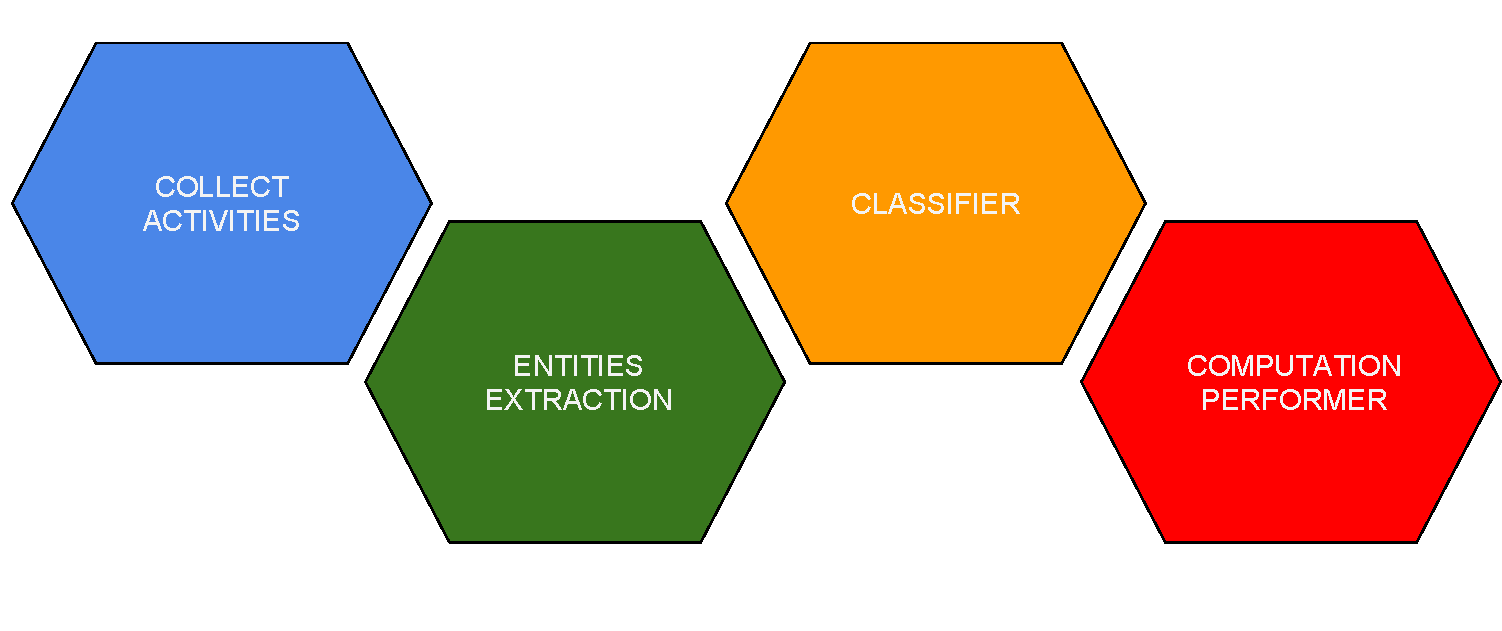
\includegraphics[width=%
0.8\textwidth]{img/Solutiondesign_nutshell}
\caption{The solution design in a nutshell.}
\label{fig:nutshell}
\end{figure}

\subsection{Collect activities}
This part has the goal to fetch user's contents on social networks, using the services for developers offered by the official APIs of each social network. The data of interest are some pieces of user's information, such as name, birthday, number of friends/followers, subscription date, his/her location and language, and of course all his/her contents: all the posts he/she wrote, with attachments, external links and the publication date, with also some other useful metadata, such us the number of likes, replies and shares. Some social media, like Twitter, offer a free API plan with some restrictions over time: for example to retrieve user's tweets is possible to make 1500 requests every 15 minutes. In case the limit is reached, this part should suspend itself waiting for a new time slot: for this reason is suggested to run this function in a dedicated thread or process.

As input this functionality needs a series of IDs that identify the user among all the social networks he/she uses, and for each social platform is necessary to know at which point the data of a given user has been downloaded. In fact, due to the huge amount of data, social network services return a small quantity of data for each request, therefore, after the first request, the point from which start to download data must be specified.

As output, a list with \textit{new} user's post is expected. In case it's the first time that the data of a user is downloaded, a list of user's information is expected too, otherwise $ n $ new posts are enough. The term \textit{new} means that all the fetched post were not previously downloaded by the system, turning out to be new for it, even if they can be dated far in the past. In other words, a new post for our system may not be new for the social network, but is simply a post that were not included in any of the previous download for that given user. Last but not least, the point the data has been fetched for the user must be updated.

The number $ n $ of post to download could be given as parameter. It would be better if the number is \textit{small}, not to overload the system. For example, Twitter allows to fetch up to $ 200 $ tweets a request. The default parameters should be setted equal to the maximum limit imposed by the API.

A possible signature of this method can be the following:

\begin{Verbatim}
[Post] CollectActivities (Integer userID, [
			    (Integer socialUserID, Integer fromPost, Integer toPost)
			   ] foreach social media to analyze
			  )
\end{Verbatim}
where \texttt{userID} is the ID into the system for the user to analyze, and an array of tuples, one for each social network the analysis will be based on, that specify the ID of the user into that specific social network, from which post to start the download and where to stop it.

\subsection{Entities extraction}
This part has the task to add semantic information to the data that was previously downloaded from social networks. What is obtained from the previous part are only raw texts and images, the goal is now to understand what the user has talked about into his/her posts. To do that, some external semantic analyzer will be used: this kind of service extracts entities, topics and sentiment starting from a text or a image. An \textit{entity} is a person, an object or a concept that has an article on Wikipedia; a \textit{topic} is a Wikipedia category to which an entity belongs to. For example, the phrase "I'm studying computer science at the university" has two entities - \texttt{Computer science} and \texttt{University} - and the following list of topics: \texttt{Electrical engineering, Electronic engineering, Computer engineering, Computer science, Educational stages, Higher education, Types of university or college, Universities and colleges, Youth}. These new metadata added to the information obtained previously will be useful in further steps to understand whether a post is about a life event or not. This functionality has also the delicate task to deal with the request rate limits of the external analyzers: in fact many of these API have strict limitations for free plans, allowing only a small amount of requests in a certain time window. In case the limit runs out, this part of the system has to suspend himself waiting for another time window to send new requests, keeping in memory all the computation requested in the meantime.

A post, composed by text, images or external links is expected as input. Furthermore, a list of posts could be accepted as input, but in this case the number of remaining requests must be handled carefully.

As output, a list of entities, topics and sentiment scores is returned for each post analyzed. The sentiment score is made by a floating point number, that ranges from a minimum value - such as $ -1.0 $ - to a maximum value - like $ 1.0 $. Instead, entities and topics can be represented by a string or an \texttt{URI}, for example a \texttt{Wikipedia URI}.

By default, everything that is returned by the external analyzer could be given as output, together with a confidence for each entity found inside texts or photos. In addition, this part of the system should provide the possibility to consider only the \textit{top entities} (e.g. the most meaningful, or those with the highest confidence), and also the possibility to set a minimum value of confidence under which the entity is discarded.

A possbile signature of this part can be the following:
\begin{Verbatim}
Post ExtractEntities (Post post)
\end{Verbatim}
which add to the post given as input the fields \textit{sentiment}, \textit{entities} and \textit{topics}.

\subsection{Classifier}
This part has the fundamental purpose to decide whether a post is about or not to a certain life event. Its task is to extract some features from the posts previously downloaded, and apply some machine learning algorithm to take this decision. As explained in section~\ref{sec:dataset}, the standard approach to classify textual contents in multiple languages is to have a great number of examples for each tongue; in this thesis a different approach is tried, using entities and topics instead of single words, for two reasons. In this way is enough to train the classifier with a single dataset in a given language $ L $ - english - and for all the contents that are not in the $ L $ language is just necessary to map all the entities in the respectives of $L$. In addition to that, with this technique is possible to consider both photos and texts as the same thing: just entity containers, it's not necessary to treat them separately. All the keys entities for a life event exist in several languages, so this mapping procedure should easily be successful: for example, the entity \texttt{Infant} for the birth of a child event exists in 82 languages. English is chosen as main language because the english version of Wikipedia has a number of articles at least 5 times bigger than any other language.

At this point the current situation is, for each user taken into analysis, a list of posts - made by texts, attachments and images - enriched with semantic entities, topics and sentiment score. The input will be a tuple (or a list of tuples) made by a post, composed as just described, and a life event of interest, for which we want to predict if the post is about it. A life event could be represented by an unique string, e.g. "\texttt{GETTING\char`_MARRIED}" for a wedding, or alternatively by an integer ID.

As output, the probabiliy with which the post (or the list of posts) concerns with the life event is expected.

The feature extraction method can be decided a priori, as described earlier, or it could be setted as parameter: in this last case is possible to use only \textit{text features} - the words that compose the text of each post - or use only \textit{entity features} - the semantic entities for reasoning on the meaning of the post, or use them both together. This choice should be made paying attention to the available datasets to train the classifier: in fact, if \textit{text features} are chosen, at least a different dataset for each language supported has to be provided as explained in section~\ref{sec:dataset}.

Two possible signatures for the classifier can be:
\begin{Verbatim}
Post predict (Post p, String lifeEvent)
[Post] predict (Post[] p, String lifeEvent)
\end{Verbatim}
with the difference that the first one works with a single post at a time, while the second one takes a list of post to classify. This function adds the attribute \textit{probability} to a post.

\subsection{Computation performer}
\label{sec:computationperformer}

\begin{figure}
\centering
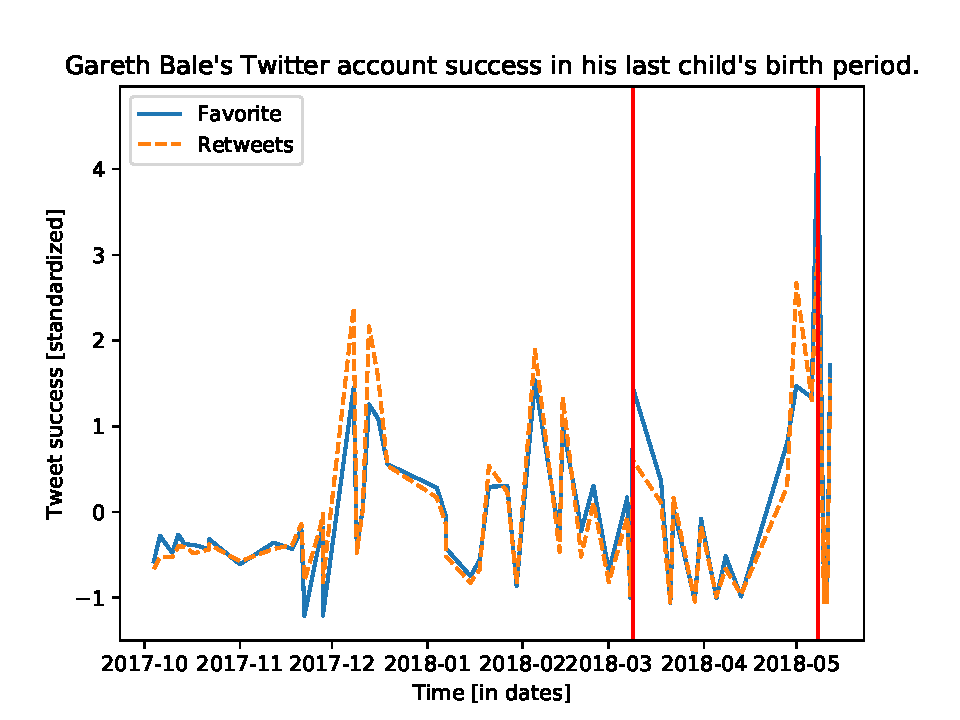
\includegraphics[width=%
0.8\textwidth]{img/bale}
\caption{The success collected by this account is high when it talks about a life event (the two red vertical line represent the pubblication of two posts related to the birth of a child).}
\label{fig:bale}
\end{figure}

This last function has the goal to analyze the user's timeline to discover a life event in it. Since a life event is something important and rare into a user's life, the assumption is that also in his/her social life his/her behaviour is different when the event is approaching or is in progress. For this reason some unusual patterns, related to the life event itself or to the average success of the posts, are searched for. The idea is that a user does not publishes contents about, for examples, a new baby, very usually, but only when something important is about to happen. In addition to that, a post about a new baby announcement gets probably more feedbacks compared to a normal post, such as congratulation messages \cite{dickinson2015identifying}. The detection of a life event is based on these routine changes, which can be various: a slow but constant increase of interest before the event, or a sudden peak when the event is happening. In general, the relative frequency of activities related to the life event itself is monitored. As shown in figure~\ref{fig:bale}, when the user talks about a life event, the success of his/her post tends to be high.
At this point, a timeline is composed by a list of post, each one with the probability of being about the life event and with the other metadata, like date of publication and post success. Let $p$ be the probability given by the classifier about a post, that post is considered related to the life event if $ p > p_1$. If the previous condition is false, but $p_2 <= p <= p_1 $, the post success is taken into consideration: let $n$ the number of post of a user, and
\[
\mu_\text{likes} = \frac{1}{n} \sum_{i=1}^n p_i.likes \quad \mu_\text{shares} = \frac{1}{n} \sum_{i=1}^n p_i.shares \quad \mu_\text{sentiment} = \frac{1}{n} \sum_{i=1}^n p_i.sentiment
\]
the average of likes, shares and sentiment among all the user's post. If 
\begin{gather}
\label{avgs}
p.likes > \mu_\text{likes} \land p.shares > \mu_\text{shares} \land p.sentiment > \mu_\text{sentiment}
\end{gather}
the post $p$ is considered related to the life event, otherwise no.

For each day $d$ the user has been active on social media (those days in which the user published something), the frequency $f$ is computed as follows:
\begin{gather}
f(d) = \frac{r(d)}{all(d)}
\label{freq}
\end{gather}
where $r(d)$ is the number of posts related to the life event written the day $d$, and $all(d)$ is the count of all posts published the day $d$. Of course, the timeline is already targeted with the life event taken into consideration. In other words, the life event to monitor is chosen in the previous steps: at this point the timeline is labelled only for a single life event. Once the frequency has been computed for every day, it can be plotted over time, and at the moment $f$ passes a given threshold $\alpha$, the life event is begun. When a minimum number of days $\beta$ in which $f(t) > \alpha$ are found, the life event can be considered as detected. By the time in $\gamma$ days there are no \textit{active days}, the life event can be seen as over.

As input is expected a list of boolean label with a timestamp, that represents the user's timeline in function to a life event.

As output, a boolean answer is expected, together with a time range in which the life event has been detected (this range can be composed by the date of the first and the last post related to the life event). Of course, the user may have not lived the life event, so in this case the list will be empty. Also, a person can live a life event more than once, so the output can be a list of labels.

There are several parameter for this phase: 
\begin{itemize}
\item a pair of probability $p_1$ and $p_2$ to consider a post directly related with the life event, or to check post success to take that decision. By default, $p_1 = 0.6$ and $p_2 = 0.4$.
\item the threshold $\alpha$ for the frequency $f$ over which the life event is considered as started.
\item $\beta$, the minimum number of \textit{active posts} to consider a life event detected. This parameter serves to correct any errors in post classification. In fact, is possible that a text or an image is misclassified: using this parameter is possible to avoid single and isolated errors.
\item $\gamma$, the maximum time between two \textit{active days} to consider them as related to the same life event. This parameter has the role to put an end to a detection, and consequently to split two consecutive life events.
\end{itemize}

A possible signature for this function is the following:
\begin{Verbatim}
[(Date from, Date to)] detectLifeEvents (Post[] posts, String Life Event)
\end{Verbatim}
where the list of post is the user's timeline, and the returned list is made of tuples, each one indicating in which period the life event has been detected.

\subsubsection{The detection algorithm}
\label{sec:computation}

In this subsection the detection algorithm, whose logic was previously explained, will be defined in pseudocode. It is assumed that all the parameters previously highlighted are defined, and that all the tree previous logical steps are already been executed. Let $n$ be the number of posts in the timeline taken into analysis, and let the data type \texttt{Post} defined as in~\ref{tab:post}.

The algorithm is composed by two main parts. In the first part, the goal is to compute the average numer of likes and shares recieved by the user among her posts, and the average sentiment score. After that, all the posts are grouped by date of publication, creating a dictionary with keys $k$ the days in which the user has published something, and values a tuple (posts related with the life event on day $k$, all posts on day $k$). This is explain in the algorithm~\ref{freq_computing}.

\begin{algorithm}
\caption{Compute the relative frequency of activities related to the life event.}
\label{freq_computing}
\begin{algorithmic}[1]
\Require posts must be sorted by date
\Function{computeFrequency}{Post[] posts}
\State $AVGLikes \gets \frac{1}{n} \sum_{i=1}^n p_i.likes $
\State $AVGShares \gets \frac{1}{n} \sum_{i=1}^n p_i.shares $
\State $AVGSentiment \gets \frac{1}{n} \sum_{i=1}^n p_i.sentiment$
\State $frequencies \gets \{\}$
\State $count \gets 0$
\State $total \gets 0$
\For{$i \gets 1 \text{ to } n$}
	\State $total \gets total + 1$
	\If{$posts[i].probability > p_1$}
		\State $count \gets count + 1$
	\ElsIf{$posts[i].probability \geq p_2 \land posts[i].likes > AVGLikes \land posts[i].shares > AVGShares \land posts[i].sentiment > AVGSentiment$}
		\State $count \gets count + 1$
	\EndIf
	\If{$i = n \lor posts[i].created \ne posts[i + 1].created$}
		\State $frequencies[posts[i].created] \gets (count, total)$
	\EndIf
\EndFor
\Return $frequencies$
\EndFunction 
\end{algorithmic}
\end{algorithm}

For each day $count$ and $total$ are computed, which represent the number of posts related to the life event and the total number of post on that day respectively. At line 10 the decision to trust the classification directly is taken. In case it's not trusted, the condition at line 12 checks whether the probabiliy is greater or equal than $p_2$ and if number of likes, shares and sentiment score are all over the average of the user, as explained in formula~\ref{avgs}. The last condition at line 14 is to understand whether a post is the last one for a day: this happens when the current post is the last one in the collection, or when the next one has a different date of creation.

In the second part the dictionary with counters is analyzed, computing for each day the frequency of activeness as in formula~\ref{freq} and analyzing it to understand if there are significant changes on it. This part is explain in the algorithm~\ref{decision}.

\begin{algorithm}
\caption{Decide whether a user has lived a life event}
\label{decision}
\begin{algorithmic}[1]
\Function{DetectLifeEvents}{frequencies}
\State $start \gets today()$
\State $end \gets \perp$
\State $count \gets 0$
\State $found \gets \{\}$
\ForAll{$k \in \text{frequencies}$}
	\State $f \gets \frac{\text{frequencies}[k].count}{\text{frequencies}[k].total}$
	\If{$f > \alpha$}
		\If{$k < start$}
			\State $start \gets k$
			\State $end \gets k$
		\EndIf
		\If{$(k - end) < \gamma$}
			\State $end \gets k$
			\State $count \gets \text{frequencies}[k].count$
		\Else
			\If{$count \geq \beta$}
				\State $found \gets found \cup \{(start, end)\}$
			\EndIf
			\State $start \gets k$
			\State $end \gets k$
			\State $count \gets 1$
		\EndIf
	\EndIf
\EndFor
\If{$count \geq \beta \land end \ne \perp$}
	\State $found \gets found \cup \{(start, end)\}$
\EndIf
\Return $found$
\EndFunction
\end{algorithmic}
\end{algorithm}

The symbol $\perp$ represents a null type. The idea is to find some time intervals that represent a life event, each one recognized by a $start$ and an $end$. For each day in which the user published something, the relative frequence $f$ is computed (at line 7) as shown in formula~\ref{freq}. If $f$ is greater than the threshold $\alpha$ and is the very first day encountered, $start$ will point to it. For every other following day in which $f > \alpha$ and that is less than $\gamma$ days later than the current $end$, $end$ is overwritten, to point to that day. When an active day is too far from the last active day, the conditions to add a life event are checked (line 16): if at least $\beta$ active posts were previously found, the life event from $start$ to $end$ is added, and these variables are restored to detect another interval. In the end, at line 21, is verified whether there is an interval left open, and in this case, if there are enough posts, a last life event is added.

The complexity of both algorithm~\ref{freq_computing} and~\ref{decision} is $\Theta(n)$ in time, because each post is analyzed only once, in both functions. 

\section{Exposed APIs}
\label{sec:APIs}

In this section the APIs offered by the system will be defined. These interfaces are RESTful APIs, which expose the main resources available in the system: \texttt{User}, \texttt{Download Request} and \texttt{Computation}. For each resource, the possibilities to retrieve and create new istances are offered, and for the user resource is also possible to edit an istance. In the following subsections more details will be provided. 

\subsection{User information {[}\protect\texttt{/user}{]}}
\label{sec:APIuser}

\subsubsection{Get a specific User {[}\protect\texttt{GET}{]}}

Get all the information about a specific user. It's possible to search using the user ID given by the system, or with the ID of a social network (At least one parameter must be specified).

\begin{itemize}
\item
  Parameters:

  \begin{itemize}
  \item
    \textit{userid}: user's identifier. (\texttt{string})
  \item
    \textit{facebookid}: user's Facebook ID. (\texttt{string})
  \item
    \textit{twitterid}: user's Twitter ID. (\texttt{string})
  \item
    \textit{instagramid}: user's Instagram ID. (\texttt{string})
  \end{itemize}
\item
  Response 200 (\texttt{application/json})

\begin{verbatim}
  {
      "ok": "true",
      "result": {
          "userid": "12dfdbGRqaS34D5Hth5PaXsw",
          "name": "Pinco Pallino",
          "twitter": {
              "name": "pincopallino",
              "id": "2565227499"
          },
          "facebook": {
              "name": "Pinco Pallino",
              "id": "2228804402"
          },
          "instagram": {
              "name": "pinco_pallino",
              "id": "388926121"
          }
      }
  }
\end{verbatim}
\item
  Response 404 (\texttt{application/json})

\begin{verbatim}
  {
      "ok": "false",
      "error": "User ID does not exist."
  }
\end{verbatim}
\end{itemize}

\subsubsection{Create a new User{[}\protect\texttt{POST}{]}}

Add a user to the system, specifying the user's IDs among the social networks to analyze. At least one social ID must be specified.

\begin{itemize}
\item
  Parameters:

  \begin{itemize}
  \item
    \textit{name}: user's name (\texttt{string, required})
  \item
    \textit{facebookid}: user's Facebook ID. (\texttt{string})
  \item
    \textit{twitterid}: user's Twitter ID. (\texttt{string})
  \item
    \textit{instagramid}: user's Instagram ID. (\texttt{string})
  \end{itemize}
\item
  Request (application/json)

\begin{verbatim}
  {
      "name": "Pinco Pallino",
      "facebookid": "2228804402",
      "twitterid": "2565227499",
      "instagramid": "388926121"
  }
\end{verbatim}
\item
  Response 200 (application/json)

\begin{verbatim}
  {
      "ok": "true",
      "result": {
          "userid": "12dfdbGRqaS34D5Hth5PaXsw",
          "name": "Pinco Pallino",
          "twitter": {
              "name": "pincopallino",
              "id": "2565227499"
          },
          "facebook": {
              "name": "Pinco Pallino",
              "id": "2228804402"
          },
          "instagram": {
              "name": "pinco_pallino",
              "id": "388926121"
          }
      }
  }
\end{verbatim}
\end{itemize}

\subsubsection{Add a social media accout to a User{[}\protect\texttt{PUT}{]}}

Add a social media account to a user, specifying the ID for the social media to add. Empty parameters will not be overwritten.

\begin{itemize}
\item Parameters:
	\begin{itemize}
	\item \textit{userid}: user's id in our system (\texttt{string, required})
	\item \textit{facebookid}: user's Facebook ID. (\texttt{string})
	\item \textit{twitterid}: user's Twitter ID. (\texttt{string})
	\item \textit{instagramid}: user's Instagram ID. (\texttt{string})
	\end{itemize}
\item
  Request (\texttt{application/json})

\begin{verbatim}
  {
      "userid": "12dfdbGRqaS34D5Hth5PaXsw",
      "twitterid": "770389450828447745"
  }
\end{verbatim}
\item
  Response 200 (\texttt{application/json})

\begin{verbatim}
  {
      "ok": "true",
      "result": {
          "userid": "12dfdbGRqaS34D5Hth5PaXsw",
          "name": "Pinco Pallino",
          "twitter": {
              "name": "therealpincopallino",
              "id": "770389450828447745"
          },
          "facebook": {
              "name": "Pinco Pallino",
              "id": "2228804402"
          },
          "instagram": {
              "name": "pinco_pallino",
              "id": "388926121"
          }
      }
  }
\end{verbatim}
\item
  Response 404 (\texttt{application/json})

\begin{verbatim}
  {
      "ok": "false",
      "error": "User ID does not exist."
  }
\end{verbatim}
\end{itemize}

\subsection{Fetch new user's activities {[}\protect\texttt{/downloadrequest}{]}}
\label{sec:APIdownloadrequest}
\subsubsection{fetch user's activities on social media not previously downloaded.{[}\protect\texttt{POST}{]}}

Request a download of activities not previously fetched. This action can take a long period to be executed, due to external service limitations. For this reason, an ID of the request is returned, to check the status of the download.

\begin{itemize}
\item
  Parameters:

  \begin{itemize}
  \item
    \textit{userid}: user's id in our system (\texttt{string, required})
  \item
    \textit{count}: number of posts to download for each social media, max 200 (\texttt{integer})
  \item
    \textit{new}: indicates if the download should retrieve activities published before di older one fetched {[}\texttt{false}{]}, or after the newer one {[}\texttt{true}{]} (\texttt{boolean string})
  \end{itemize}
\item
  Request (\texttt{application/json})

\begin{verbatim}
  {
      "userid": "12dfdbGRqaS34D5Hth5PaXsw",
      "count": 200,
      "new": "false"
  }
\end{verbatim}
\item
  Response 200 (\texttt{application/json})

\begin{verbatim}
  {
      "ok": "true",
      "fetchid": "5adFgtu23_564aSbmogr346h0q"
  }
\end{verbatim}
\end{itemize}

\subsubsection{Check the status of an activity fetch request.{[}\protect\texttt{GET}{]}}

Check whether a previous request was satisfied or is still waiting to be executed.

\begin{itemize}
\item
  Parameters:

  \begin{itemize}
  \item
    \textit{fetchid}: the ID of a fetch request previously done. (\texttt{string, required})
  \end{itemize}
\item
  Response 200 (\texttt{application/json})

\begin{verbatim}
  {
      "ok": "true",
      "status": "completed" <!-- The status can be "in progress", or "waiting" -->
  }
\end{verbatim}
\item
  Response 404 (\texttt{application/json})

\begin{verbatim}
  {
      "ok": "false",
      "error": "Fetch request ID does not exist."
  }
\end{verbatim}
\end{itemize}

\subsection{Detect a life event into a user timeline. {[}\protect\texttt{/computation}{]}}
\label{sec:APIcomputation}

Endpoint to request and get a computation to detect a specific life event into a user's timeline.

\subsubsection{Request a computation. {[}\protect\texttt{POST}{]}}

Request a computation of a user timeline to discover a life event.

\begin{itemize}
\item
  Parameters:

  \begin{itemize}
  \item
    \textit{userid}: user's id in our system (\texttt{string, required})
  \item
    \textit{lifeevent}: the life event to search for (\texttt{string}, it can be "\texttt{GETTING\_MARRIED}" or "\texttt{HAVING\_CHILDREN}")
  \end{itemize}
\item
  Request (\texttt{application/json})

\begin{verbatim}
  {
      "userid": "12dfdbGRqaS34D5Hth5PaXsw",
      "lifeevent": "GETTING_MARRIED"
  }
\end{verbatim}
\item
  Response 200 (\texttt{application/json})

\begin{verbatim}
  {
      "ok": "true",
      "computationid": "5add910030cb954661f458f4"
  }
\end{verbatim}
\end{itemize}

\subsubsection{Get the result of a computation {[}\protect\texttt{GET}{]}}

Get a computation previously requested.

\begin{itemize}
\item
  Parameters:

  \begin{itemize}
  \item
    \textit{computationid}: the ID of the computation to get (\texttt{string, required})
  \end{itemize}
\item
  Response 200 (\texttt{application/json})

\begin{verbatim}
  {
      "ok": "true",
      "result": {
          "computationid": "5add910030cb954661f458f4",
          "userid": "12dfdbGRqaS34D5Hth5PaXsw",
          "lifeevent": "GETTING_MARRIED",
          "detection": [
              {
                  "from": "2015-12-4",
                  "to": "2016-8-15"
              }
          ]
      }
  }
\end{verbatim}

\item
  Response 404 (\texttt{application/json})

\begin{verbatim}
  {
      "ok": "false",
      "error": "Computation ID does not exist."
  }
\end{verbatim}
\end{itemize}

\section{Global view}

\begin{figure}
\centering
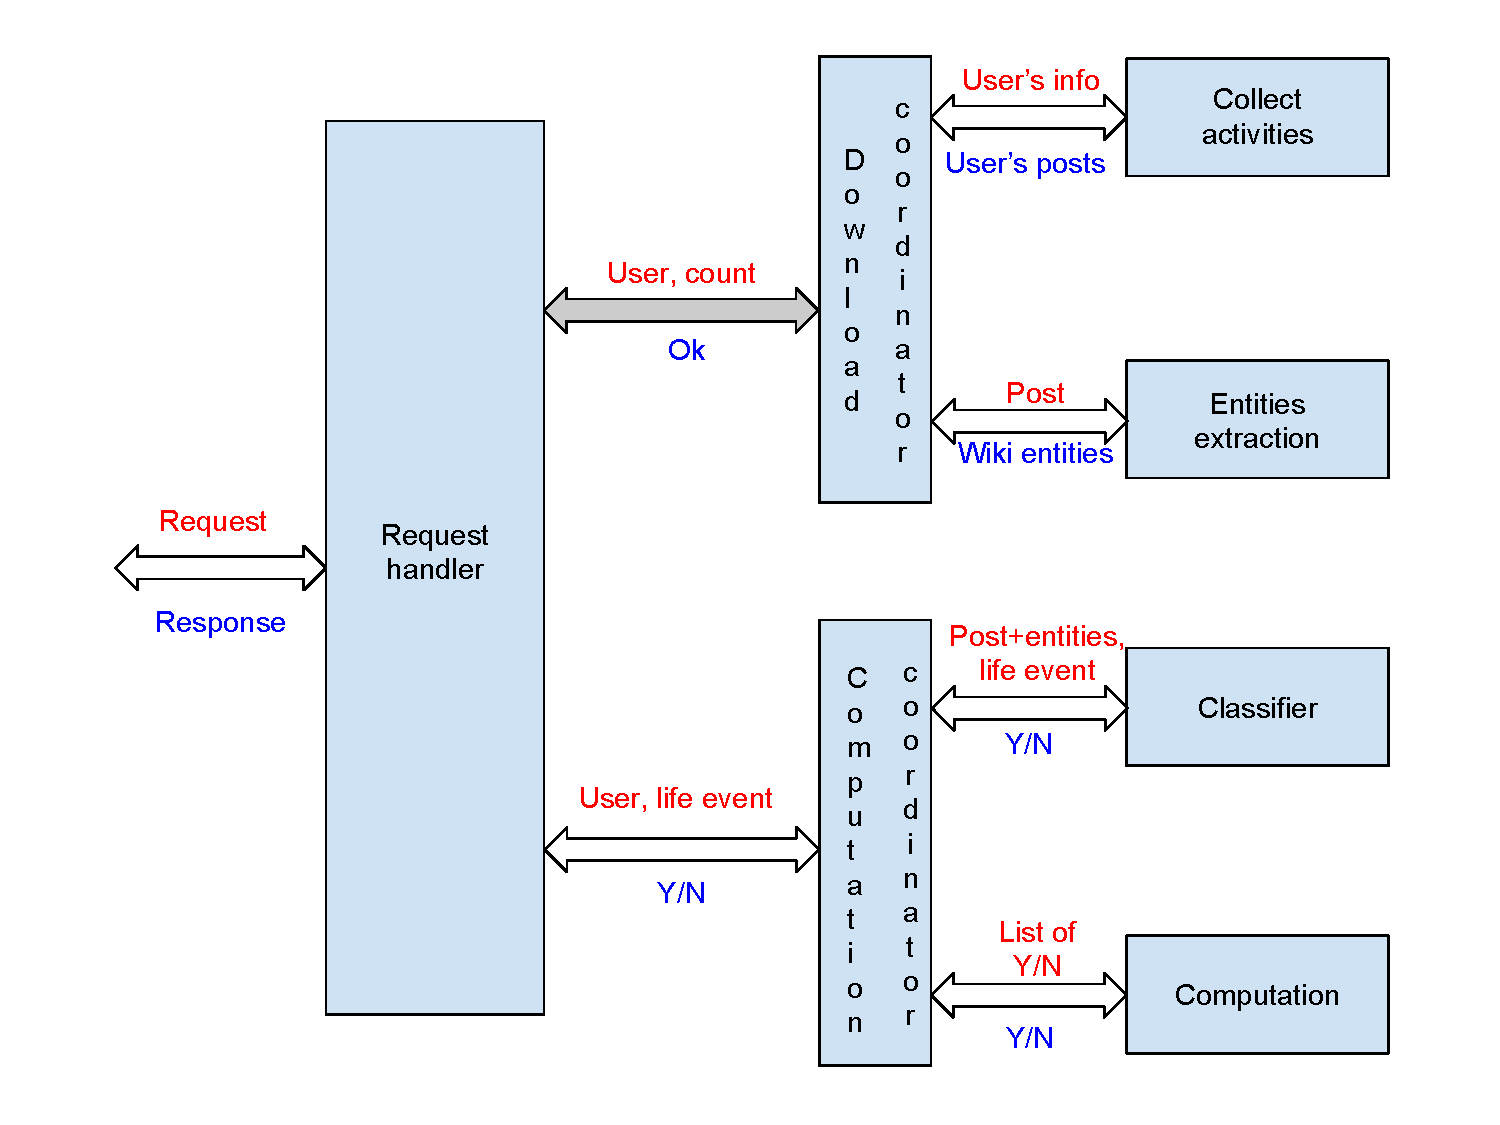
\includegraphics[width=%
1.0\textwidth]{img/Globalview}
\caption{A global view of the system with the data exchanged between the components. Grey arrows are queues of inputs, while white arrows are messagges of a class method call.}
\label{fig:globalview}
\end{figure}

Overall, the composition of the system can be divided in two big parts: the one to get the data, the other to analyze the data. The four logical steps previously explained in section~\ref{sec:design} are translated into four components placed in the deepest point of each request, as shown in figures~\ref{fig:globalview} and \ref{fig:interaction}. These four parts have different roles and behaviours: some of them are autonomous, while some others depend one from the other.

\begin{figure}
\centering
\includegraphics[width=%
0.95\textwidth]{img/Interaction}
\caption{The interaction among components over time.}
\label{fig:interaction}
\end{figure}

The first block is the user's endpoint of the system, the only access point from the outside. It has the role to handle the APIs described in section~\ref{sec:APIs} and to call the functions in order to fulfill the requests it receives. In case of a \texttt{/user} request, it's able to respond to it independently, just accessing the internal database. Contrariwise, when a download or a computation is requested, its role is to understand the data situation for the object of the request and to launch the right component to satisfy it.

The download request will be described in detail in section~\ref{sec:downloadqueues}.

The computation request is much easier, because it only works with data within the system, without any external service. Each request is fulfilled with the personal data of the user in analysis present at the time of the request. This process can be seen in the lower part of picture~\ref{fig:globalview}. User's posts are firstly classified as related or not to the life event taken into analysis, and then data is given to the computator part to detect any life event into user's timeline, as explained in section~\ref{sec:computation}. 

\subsection{A queue system to download user's contents}
\label{sec:downloadqueues}

\begin{figure}
\centering
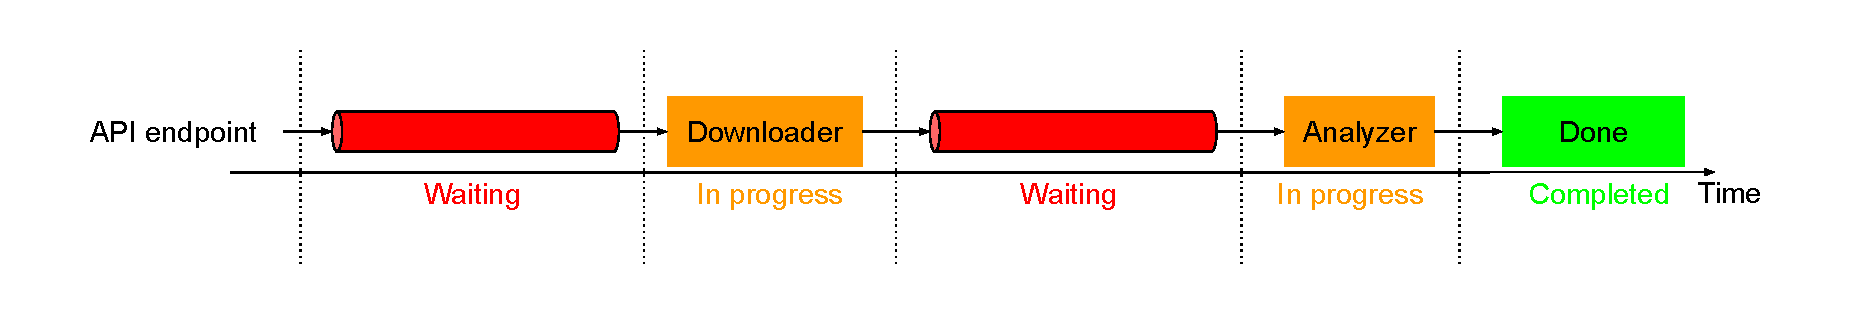
\includegraphics[width=%
1\textwidth]{img/DownloadStatuses}
\caption{The changing of status over time of a download request.}
\label{fig:statuses}
\end{figure}

\begin{figure}
\centering
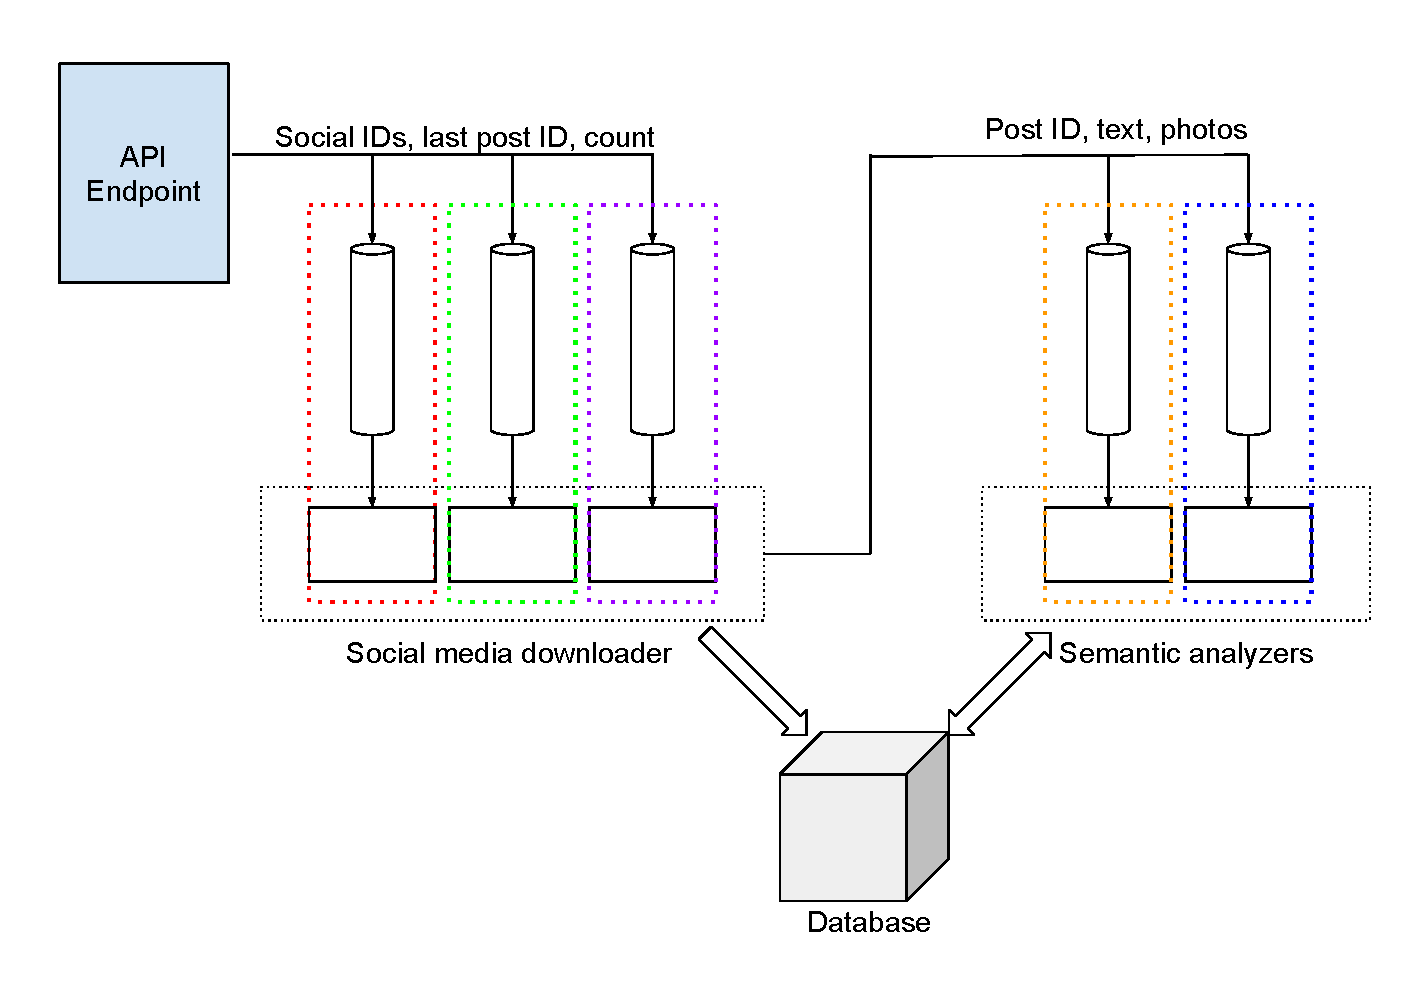
\includegraphics[width=%
1\textwidth]{img/Queues}
\caption{The route of a download request. From the endpoint, data is divided in indipendent streams, one for each social media, and each stream is enqueued in the corresponding queue. The red, green and purple frames represents three different social network download system -- for example the red one for Facebook, the green one for Twitter and the purple one for Instagram. Once data is downloaded, it is saved into the database, and posts are given to the semantic analyzers, represented by the orange and blue frames: one for texts and one for images.}
\label{fig:queues}
\end{figure}

The most complex request is a \texttt{/downloadrequest}, because it has to face with external APIs over HTTPS, which have free plans with request limits over a time range. Due to this issue, each part needed to fulfill this kind of requests has to be able to suspend itself without interrupt the whole system. In other words, when the function for downloading contents on a social network, or the one that deals with the external semantic analyzer reaches the limit of requests, it has to wait for another time slot stopping only itself and nothing else. For this reason data is not passed with a standard class method call, but they are inserted into a queue. There will be a queue for each module that has to interface itself with an external service, so one for each social media and one for every semantic analyzer (one for texts and one for pictures). This decision is necessary to avoid bottlenecks as much as possible: in case a social network API reaches the limit, the download in the other social networks can be carried on, and so also the following requests can start. The only thing that is necessary is to track when each part of the Download Request finishes, in order to have always a current status for every request of download: when at least a data stream of a request is taken over by the downloader or the analyzer, the status is \textit{in progress}, while if all data streams of a requests are waiting into a queue, the status is \textit{waiting}. By the time each stream passed into its specific downloader and analyzer, the status will be \textit{completed}. The status timeline can be seen in picture~\ref{fig:statuses}.

For example, let's suppose to download contents made by a user who is signed up to Twitter, Facebook and Instagram. The request will be collected by the API endpoint, which will verify if the user exists into the database of the system, and in case it exists the endpoint will get from the same database, for each of the three social media, the user ID and the last post downloaded in a previous request, if there is one. After that, the tuple (user ID, starting point, number of post to download) is queued in the respective social media queue, and an immidiate response is given to the API request, to let the user know that her request has taken into consideration. At this point, each stream of data (one for each social media) will go on indipendently: it will wait its turn into the downloader queue, then data will be downloaded and saved into the database, then for each downloaded post, the tuples (post ID, text) and (post ID, photos) will be enqueued in the text semantic analyzer and in the image semantic analyzer respectively. When all these streams will have passed both downloader and analyzers, the request will be completed. This schema can be seen in picture~\ref{fig:queues}.

Even though this architecture avoids as much as possible bottlenecks, a download request can take a very long time to be completed (even days), because each post from any social media has to pass through the semantic analyzers, which have a very restricted number of requests a day.

